\message{ !name(main.tex)}%%%%%%%%%%%%%%%%%%%%%%%%%%%%%%%%%%%%%%%%%
% fphw Assignment
% LaTeX Template
% Version 1.0 (27/04/2019)
%
% This template originates from:
% https://www.LaTeXTemplates.com
%
% Authors:
% Class by Felipe Portales-Oliva (f.portales.oliva@gmail.com) with template 
% content and modifications by Vel (vel@LaTeXTemplates.com)
%
% Template (this file) License:
% CC BY-NC-SA 3.0 (http://creativecommons.org/licenses/by-nc-sa/3.0/)
%
%%%%%%%%%%%%%%%%%%%%%%%%%%%%%%%%%%%%%%%%%

%----------------------------------------------------------------------------------------
%	PACKAGES AND OTHER DOCUMENT CONFIGURATIONS
%----------------------------------------------------------------------------------------

\documentclass[
	12pt, % Default font size, values between 10pt-12pt are allowed
	%letterpaper, % Uncomment for US letter paper size
	%spanish, % Uncomment for Spanish
]{fphw}

% Template-specific packages
\usepackage[utf8]{inputenc} % Required for inputting international characters
\usepackage[T1]{fontenc} % Output font encoding for international characters
\usepackage{mathpazo} % Use the Palatino font
\usepackage{amssymb}
\usepackage{graphicx} % Required for including images

\usepackage{booktabs} % Required for better horizontal rules in tables

\usepackage{listings} % Required for insertion of code

\usepackage{enumerate} % To modify the enumerate environment
\usepackage[super]{nth}
% ----------------------------------------------------------------------------------------

%	ASSIGNMENT INFORMATION
%----------------------------------------------------------------------------------------


\title{IA LAB: Ladder Logic Programmes} % Assignment title
\author{Darsh Gajjar} % Student name

\institute{SVNIT, SURAT \\ M. Tech. I \& C (Electrical Department)} % Institute or school name

\class{Industrial Automation LAB} % Course or class name

\professor{Dr. H. G. Patel} % Professor or teacher in charge of the assignment

%----------------------------------------------------------------------------------------

\begin{document}

\message{ !name(main.tex) !offset(-3) }


\maketitle % Output the assignment title, created automatically using the information in the custom commands above

%----------------------------------------------------------------------------------------
%	ASSIGNMENT CONTENT
%----------------------------------------------------------------------------------------

\section*{Program \#1}

\begin{problem}
\medskip
	There is Big godown in which there are 3 sensors installed,
 \renewcommand{\labelitemi}
 {$\blacksquare$}
 \begin{itemize} 
    \item If any one sensor is on then indicators ON,
    \item If any two sensors on then hooters ON,
    \item If all sensors are ON then Fire extinguisher should be ON
  \end{itemize} 
\end{problem}
%------------------------------------------------
\subsection*{Answer}
 \begin{center}
 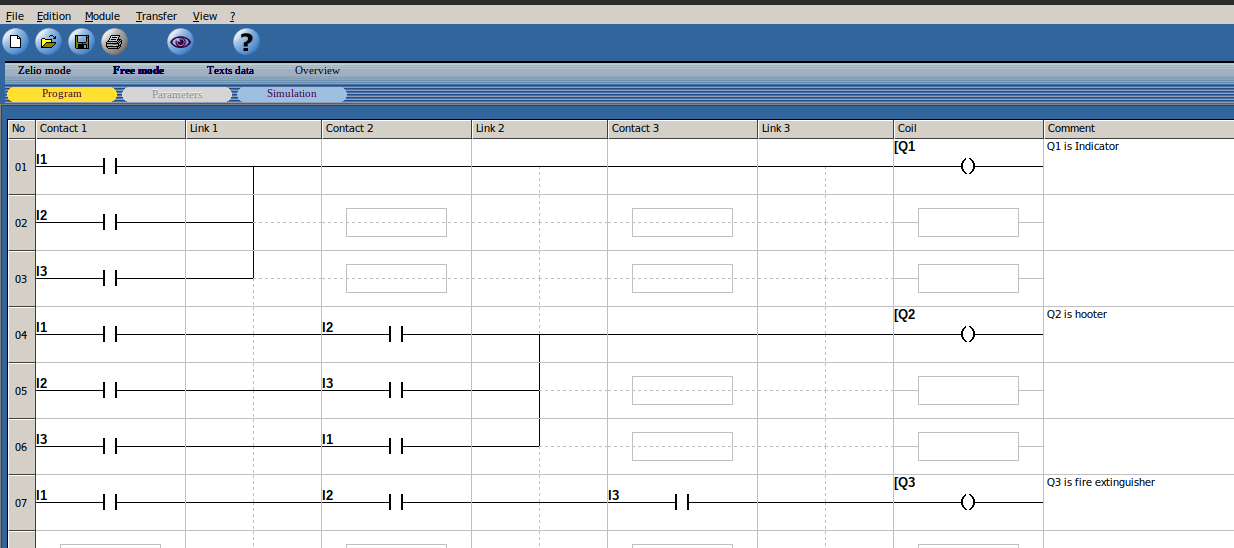
\includegraphics[width=165mm, scale=0.80]{prg1.png} % Example image
 \end{center}
%----------------------------------------------------------------------------------------
\section*{Program \#2}
\medskip
 One cutting machine with left and right start switches
 \renewcommand{\labelitemi}
 {$\blacksquare$}
  \begin{itemize}%[(\itshape a\normalfont)]
    \item If both switches on then machine on
    \item When you release any switch machine off
  \end{itemize}
  \subsection*{Answer}
  \begin{center}
    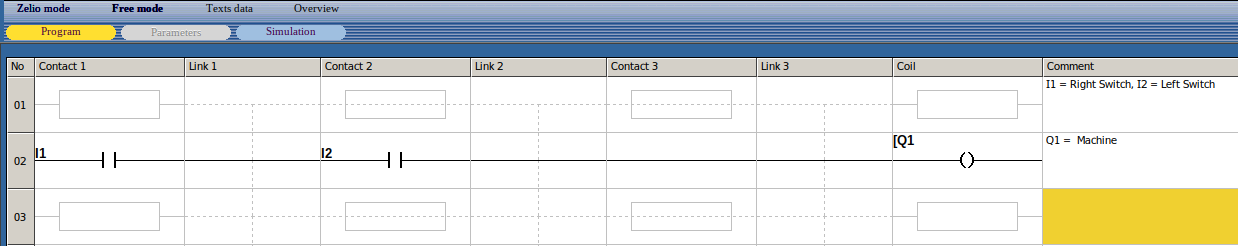
\includegraphics[width=165mm, scale=0.80]{prg2.png}
  \end{center}
  % -------------------------------------------------------------------------------------------------------
\section*{Program \#3}
\medskip

\begin{problem}
 whenever we press ON Push button then Motor should remain ON and when STOP
 push button is press it shoulf OFF immediately
\end{problem}

\subsection*{Answer}
  \begin{center}
    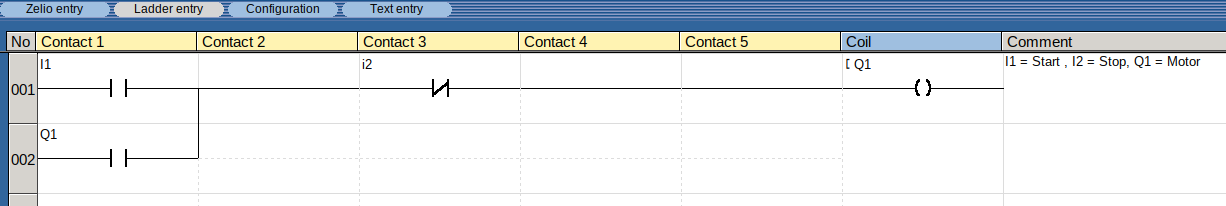
\includegraphics[width=165mm, scale=0.80]{prg3.png}
  \end{center}
  % -----------------------------------------------------------------------------------------------------------------------
\section*{Program \#4}
\medskip
\begin{problem}
  In 35 feet long machine design ladder logic by which operator should able to
  Start and Stop from three different place 
\end{problem}

\subsection*{Answer}
\begin{center}
  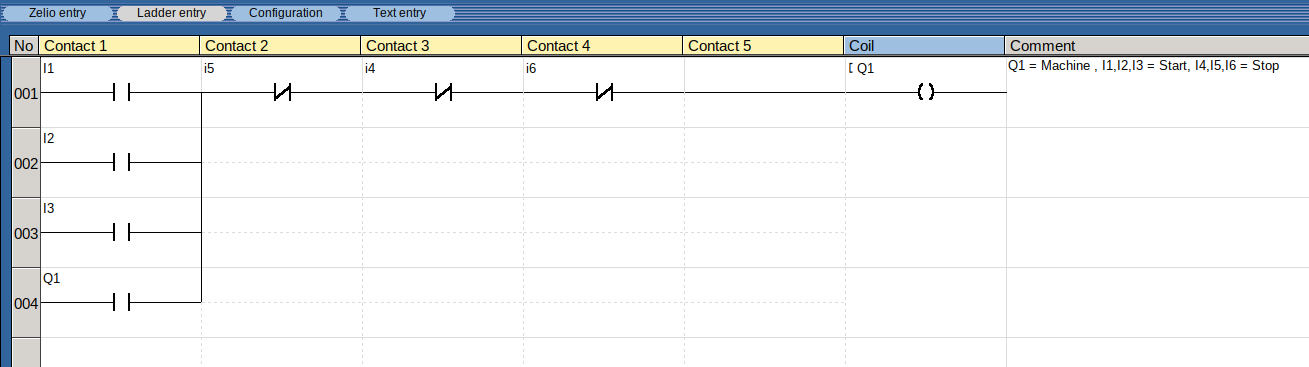
\includegraphics[width=165mm, scale=0.80]{prg4.png}
\end{center}
% ---------------------------------------------------------------------------------------------------------------
\section*{Problem \#5}
\medskip
\begin{problem}
  There is one lubrication Pump and one Motor
 {$\blacksquare$}
  \begin{itemize}%[(\itshape a\normalfont)]
    \item first lubrication Pump should be On and then Motor ON
    \item When STOP Push button is pressed Motor and Pump should be Stop together 
  \end{itemize}
\message{ !name(main.tex) !offset(-136) }
